\documentclass{article} % For LaTeX2e
\usepackage{nips15submit_e,times}
\usepackage{hyperref}
\usepackage{url}
\usepackage{graphicx}
\usepackage{amsmath}
%\documentstyle[nips14submit_09,times,art10]{article} % For LaTeX 2.09


\title{Awesome work on Machine Learning and Finite Element Models}


%\author{
%David S.~Hippocampus\thanks{ Use footnote for providing further information
%about author (webpage, alternative address)---\emph{not} for acknowledging
%funding agencies.} \\
%Department of Computer Science\\
%Cranberry-Lemon University\\
%Pittsburgh, PA 15213 \\
%\texttt{hippo@cs.cranberry-lemon.edu} \\
%\And
%Coauthor \\
%Affiliation \\
%Address \\
%\texttt{email} \\
%\AND
%Coauthor \\
%Affiliation \\
%Address \\
%\texttt{email} \\
%\And
%Coauthor \\
%Affiliation \\
%Address \\
%\texttt{email} \\
%\And
%Coauthor \\
%Affiliation \\
%Address \\
%\texttt{email} \\
%(if needed)\\
%}

% The \author macro works with any number of authors. There are two commands
% used to separate the names and addresses of multiple authors: \And and \AND.
%
% Using \And between authors leaves it to \LaTeX{} to determine where to break
% the lines. Using \AND forces a linebreak at that point. So, if \LaTeX{}
% puts 3 of 4 authors names on the first line, and the last on the second
% line, try using \AND instead of \And before the third author name.

\newcommand{\fix}{\marginpar{FIX}}
\newcommand{\new}{\marginpar{NEW}}

%\nipsfinalcopy % Uncomment for camera-ready version

\begin{document}


\maketitle

%\begin{abstract}
%\end{abstract}

\section{Finite Element Methods}

\subsection{Physics of Elastic Objects}

The simulation of deformable elastic solids has become a rich field of research due to its usefulness in computer animation and graphics. The Finite Element Method (FEM) is the most popular tool to address this problem due to its versatility in representing elastic bodies with intricate geometric features and diverse material properties. 

To understand FEM, the first step is understanding what it means for an object to be deformed due to some external forces and to its elastic properties. A thorough analysis of the physics laws of deformable objects is out of the scope of this work, the interested reader can refer to [REF] for more details. From a very high level perspective, each object occupies a precise volume $\Omega$ in a specific coordinate system. Due to external forces, the object can be subject to deformation, i.e. each material point $\overrightarrow{X} \in \Omega$ will be displaced to a \emph{new} deformed location $\overrightarrow{x}$. Typically, this deformation is defined by a \emph{deformation map} $\phi(\overrightarrow{X}) = \overrightarrow{x}$ (see Figure \ref{fig:def_map}).

One of the consequences of elastic deformation is the accumulation of potential energy  in the deformed body. This energy is often defined as $E[\phi]$, to suggest that it is fully determined by the deformation map of a given object. More precisely, different parts of a deforming object undergo shape changes in of different severity. As a consequence, the relation between deformation and energy is better defined on a local scale. We introduce the energy density function $\Psi[\phi ; \overrightarrow{X}]$ which measures the energy per unit of deformed volume on an infinitesimal volume $dV$ around the material point $\overrightarrow{X}$. We can define the total energy of the deforming body, by integrating over the entire object volume $\Omega$: 

\begin{equation}
E[\phi] =  \int_{\Omega} \Psi [ \phi ; \overrightarrow{X} ] d\overrightarrow{X}
\label{eq:energy-eq}
\end{equation}

Without going into the full details, it is possible to write $\Psi[\phi ; \overrightarrow{X}] = \Psi ( \mathbf{F} (\overrightarrow{X}) )$, where $\mathbf{F}$ is the Jacobian of the deformation map, referred to as the deformation gradient, calculated at a specific material point $\overrightarrow{X}$. This definition of the energy density function is necessary to introduce properties related to the material models of a specific object, i.e., the precise mathematical expression of $\Psi(\mathbf{F})$ will be the defining property of the material model\footnote{We will not provide here concrete examples of material models and their corresponding energy definition. The reader can refer to [REF] for more details.}. 

\begin{figure}
\centering
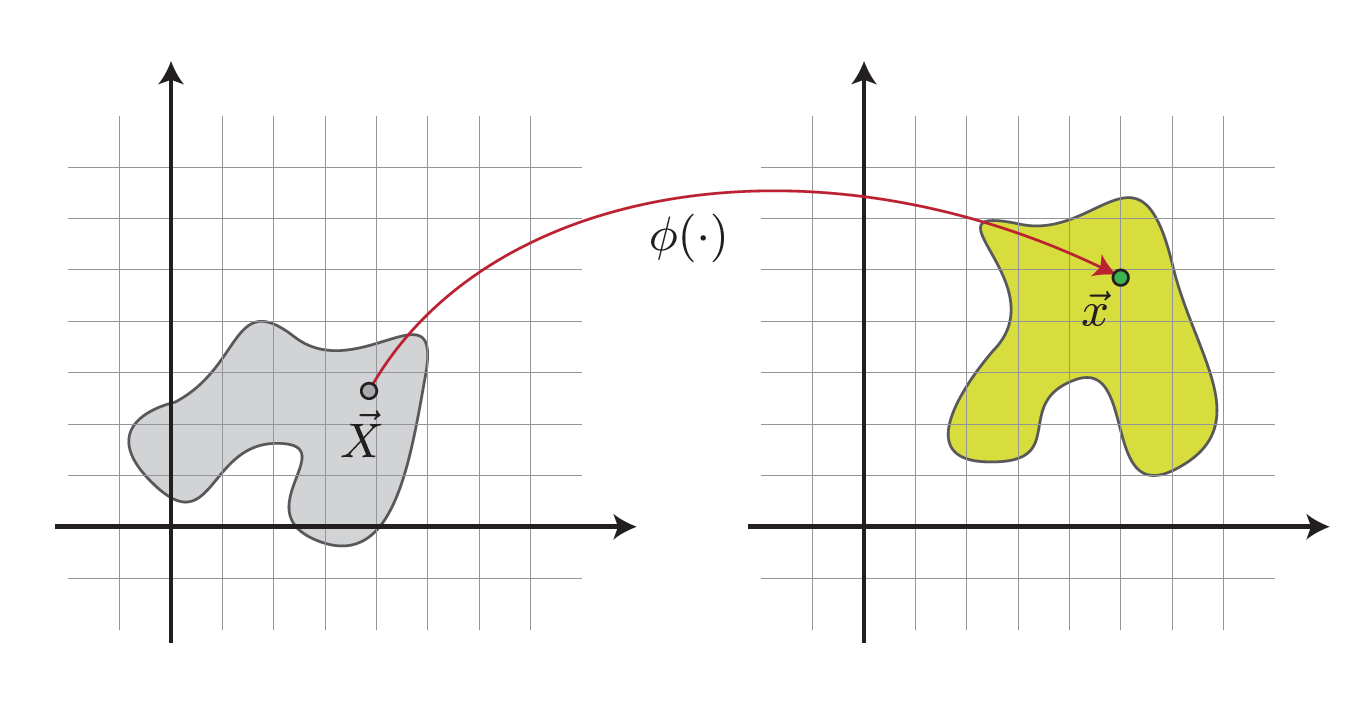
\includegraphics[width=0.75\linewidth]{figures/deformation_map.eps}
\label{fig:def_map}
\caption{Example of the deformation map}
\end{figure}

\subsection{Discretization}

In order to enable numerical simulation, the physical laws introduced in the section above need to be discretized. Elastic energy and elastic forces (which we will describe below) need to be reformulated as functions of discrete state variables. 

\subsection{Elastic Forces}\label{sec:el-forces}

When modeling a deformable body on a computer, we only store the values of the deformation map $\phi( \overrightarrow{X} )$ on a finite number of points $\overrightarrow{X}_1, \overrightarrow{X}_2, \overrightarrow{X}_3, \dots, \overrightarrow{X}_N$ corresponding to the vertices of a discretization mesh. The respective deformed vertex locations $\overrightarrow{x}_i = \phi(\overrightarrow{X}_i),\ i = 1, 2, \dots, N$ are defined as the degrees of freedom of the problem. The idea is then to specify a method to reconstruct a continuous deformation map $\hat{\phi}$, from the discrete samples $\overrightarrow{x}_i = \phi(\overrightarrow{X}_i)$, i.e., by defining a specific interpolation scheme. We denote the interpolated deformation map as $\hat{\phi}[\overrightarrow{X}; \mathbf{x}]$, which emphasizes the dependency on the discrete state $\mathbf{x} = (\overrightarrow{x}_1, \overrightarrow{x}_2 , \dots, \overrightarrow{x}_N )$. 

We can define the discrete Energy, as a function of the degrees of freedom $\mathbf{x}$, by simply plugging the interpolated deformation $\hat{\phi}$ into the definition of the standard energy:

\begin{equation}
E(\mathbf{x} ) := E \left[  \hat{\phi}(\overrightarrow{X}; \mathbf{x}) \right] = \int_{\Omega} \Psi \left( \hat{\mathbf{F}}(\overrightarrow{X}; \mathbf{x}) \right)
\label{eq:disc-energy}
\end{equation}

where $\hat{\mathbf{F}}(\overrightarrow{X}; \mathbf{x}) = \partial\hat{\phi}(\overrightarrow{X}; \mathbf{x}) / \partial\overrightarrow{X}$ is the deformation gradient computed from the interpolated map $\hat{\phi}$.

Having defined the discrete energy $E(\mathbf{x})$ we can now compute the elastic forces associated with individual mesh nodes, by taking the negative gradient of the elastic energy with respect to the corresponding degree of freedom: 

$$ \overrightarrow{f_i}(\mathbf{x}) = \frac{\partial E(\mathbf{x})}{\partial\overrightarrow{x}_i}\quad \text{or, collectively}\quad \mathbf{f} := (\overrightarrow{f_1}, \overrightarrow{f_2}, \dots, \overrightarrow{f_N}) = - \frac{\partial E(\mathbf{x})}{\partial \mathbf{x}}$$

In practice, before computing each force, the energy integral in Equation \ref{eq:disc-energy}  is separated into the contributions of the individual elements $\Omega_e$ as follows: 

\begin{equation}
E(\mathbf{x}) = \sum_e E^e (\mathbf{x}) = \sum_e \int_{\Omega_e} \Psi ( \hat{ \mathbf{F} }( \overrightarrow{X}; \mathbf{x} )  ) d\overrightarrow{X}
\label{eq:tetra-energy}
\end{equation} 

In our work, without losing generality, we will focus on linear tetrahedra, which are among the most popular discrete volumetric representations and which offer on of the most straightforward option for constructing a discretization of the elasticity equations, i.e. the reconstructed deformation map $\hat{\phi}$ can be defined as a \emph{piecewise linear function} over each tetrahedron. Specifically, for each tetrahedron $\mathcal{T}_i$ we have:

\begin{equation}
\hat{\phi} ( \overrightarrow{X} )= \mathbf{A}_i\overrightarrow{X} + \overrightarrow{b}_ i\quad \text{for all}\quad \overrightarrow{X} \in \mathcal{T}_i
\label{eq:tetra-interpol}
\end{equation}  

Figure \ref{fig:tetrahedron} shows an example of a tetrahedron. Differentiating Equation \ref{eq:tetra-interpol} with respect to $\overrightarrow{X}$ reveals that the deformation gradient $\mathbf{F} = \partial \hat{\phi} / \partial \overrightarrow{X} = \mathbf{A}_i$ is a constant on each element. Thus, for simplicity we can write $\hat{\phi} ( \overrightarrow{X} )= \mathbf{F}\overrightarrow{X} + \overrightarrow{b}_ i$.  Then, since $\mathbf{F}$ is constant, the energy of a single tetrahedron can be rewritten (after some manipulation) as 

\begin{equation}
E_i = \int_{\mathcal{T}_i} \Psi(\mathbf{F}) d\overrightarrow{X} = \Psi(\mathbf{F}_i)\int_{\mathcal{T}_i} d\overrightarrow{X} = W \cdot \Psi(\mathbf{F}_i)\quad \text{or}\quad  E(\mathbf{x}) = W \cdot \Psi(\mathbf{F}(\mathbf{x}))
\label{eq:tetra-energy-simplified}
\end{equation}

We can then use Equation \ref{eq:tetra-energy-simplified} to derive the contribution of element $\mathcal{T}_i$ to the elastic forces on its four vertices  as $f^i_k = - \partial E_i(\mathbf{x}) / \partial \overrightarrow{x}_k$.

\begin{figure}
\centering
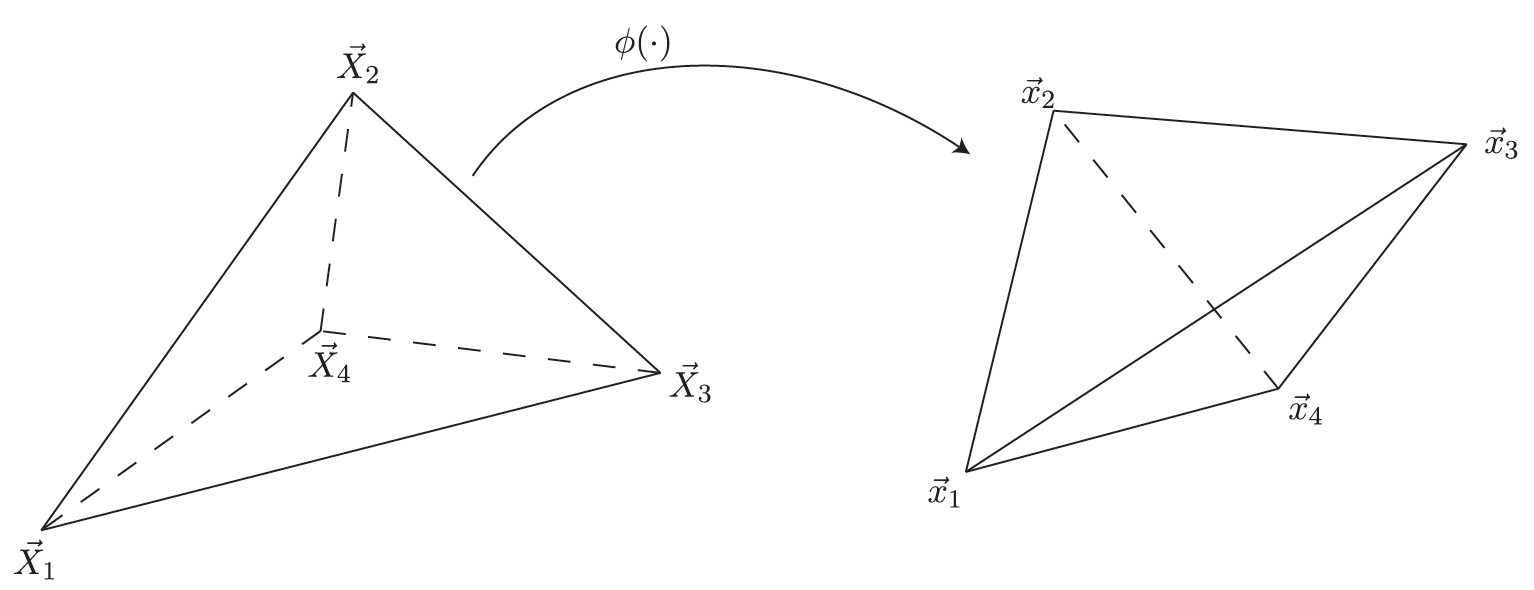
\includegraphics[width=0.75\linewidth]{figures/tetrahedron.eps}\label{fig:tetrahedron}\caption{A tetrahedron before and after a deformation}
\end{figure}

\subsection{Forces Differentials}\label{sec:force-diff}

The most common integration scheme used to simulate elastic objects is the Backward Euler method. At any moment in time, this method simulates the action of a force over a vertex of an element of a deformable object. To do so, in addition to discrete nodal forces it also requires a process to compute \emph{force differentials}, i.e., linearized nodal force increments around a configuration $\mathbf{x}_{*}$, relative to a small nodal force displacement $\delta \mathbf{x}$. We denote this by:

\begin{equation}
\delta \mathbf{f} = \delta \mathbf{f}(\mathbf{x}_{*}; \delta\mathbf{x}) := \frac{\partial \mathbf{f}}{\partial \mathbf{x}} \Bigg |_{\mathbf{x} = \mathbf{x}_{*}} \cdot \delta \mathbf{x}
\label{eq:force-diff}
\end{equation} 

The expression in Equation \ref{eq:force-diff} makes use of the stiffness matrix $\partial \mathbf{f} / \partial \mathbf{x} $, which is typically hard to calculate. Instead, the aim is to compute the force differential vector $\delta \mathbf{f}$ on an element-by-element basis, accumulating the contribution of each element to the aggregate value of each of its nodes. This is done using only the information in the current state $\mathbf{x}_{*}$, the displacement $\delta \mathbf{x}$ and a small amount of additional meta-data (see [REF] for the specific derivation).

\section{The Backward Euler Method}

Given the background described in the previous section, we can now describe a complete implicit-time integration scheme for non-linear elastic bodies. In order to define the backward Euler integrations scheme (BE), we need to maintain both the position ($\mathbf{x}^n$) and the velocity ($\mathbf{v}^n$) of the deforming body at time $t^n$. The BE scheme calculate the position $\mathbf{x}^{n+1}$ and velocity $\mathbf{v}^{n+1}$ at time $t^{n+1}$(:= $t^{n+1} + \Delta t$) as the solution of the following non-linear system of equations: 

\begin{align}
\mathbf{x}^{n+1} &= \mathbf{x}^n + \Delta t \mathbf{v}^{n + 1}\label{eq:non-linearity-1}\\
\mathbf{v}^{n+1} &= \mathbf{v}^n + \Delta t \mathbf{M}^{-1} \mathbf{f}(\mathbf{x}^{n+1}, \mathbf{v}^{n+1})\nonumber\\
			  &= \mathbf{v}^n + \Delta t \mathbf{M}^{-1} \left ( \mathbf{f}_e(\mathbf{x}^{n+1}) + \mathbf{f}_d( \mathbf{x}^{n+1}, \mathbf{v}^{n+1} ) \right )\label{eq:non-linearity-2}
\end{align}
where we introduce the following notation:
\begin{itemize}
\item $\mathbf{f}_e( \mathbf{x}_{*} )$: Elastic forces at configuration $\mathbf{x}_{*}$, as defined in Section \ref{sec:el-forces}.
\item $\mathbf{f}_d( \mathbf{x}^*, \mathbf{v}^* ) = -\gamma \mathbf{K}(\mathbf{x}^*) \mathbf{v}^*$: damping forces at position $\mathbf{x}^*$ and velocity $\mathbf{v}^*$ according to the Rayleigh damping model. $\gamma$ does not have a predefined range. 
\item $\mathbf{K}(\mathbf{x}^*) = \frac{\partial \mathbf{f}_e}{\partial \mathbf{x}} \big |_{\mathbf{x}^*}$ is the elasticity stiffness matrix evaluated at $\mathbf{x}^*$. This matrix is typically constructed using the force differential defined in Section \ref{sec:force-diff}. 
\item $\mathbf{f}( \mathbf{x}^*, \mathbf{v}^* ) = \mathbf{f}_e( \mathbf{x}_{*} ) + \mathbf{f}_d( \mathbf{x}^*, \mathbf{v}^* )$: aggregate forces including elastic and damping constraints. 
\item $\mathbf{M}$: the mass matrix.
\end{itemize}

Now, Equation \ref{eq:non-linearity-2} makes the Backward Euler system non-linear. To address this issue, an iterative process is defined to compute the unknowns $\mathbf{x}^{n+1}$ and $\mathbf{v}^{n+1}$, such that the approximations converge to the real value as the number of iterations goes to infinity: $\mathbf{x}^{n+1}_{(k)} \rightarrow_{k \rightarrow \infty} \mathbf{x}^{n+1}$ and $\mathbf{v}^{n+1}_{(k)} \rightarrow_{k \rightarrow \infty} \mathbf{v}^{n+1}$ (the initial guesses will be the position and velocity of the previous step). We define the position and velocity correction variables as:
 
 $$\Delta \mathbf{x}_{(k)} := \mathbf{x}^{n+1}_{(k+1)} -  \mathbf{x}^{n+1}_{(k)}\quad \text{and}\quad \Delta \mathbf{x}_{(k)} := \mathbf{v}^{n+1}_{(k+1)} - \mathbf{v}^{n+1}_{(k)}$$

The key idea of the correction scheme is the following: at each step of the iterative scheme, Equations \ref{eq:non-linearity-1} and \ref{eq:non-linearity-2} are linearized around the current iterate ($\mathbf{x}^{n+1}_{(k)}, \mathbf{v}^{n+1}_{(k)}$). The solutions of such linearization are then used to define the next iterate ($\mathbf{x}^{n+1}_{(k+1)}, \mathbf{v}^{n+1}_{(k+1)}$). Referring to [REF], for further details, using some mathematical manipulation, we linearize Equation \ref{eq:non-linearity-2} as:

\begin{align}
\mathbf{v}^{n+1}_{(k)} + \Delta \mathbf{v} &=\nonumber\\ 
\mathbf{v}^n + &\Delta t \mathbf{M}^{-1} \left (  \mathbf{f}_e ( \mathbf{x}^{n+1}_{(k)} ) + \frac{\partial \mathbf{f}_e}{\mathbf{x}} \big |_{\mathbf{x}^{n+1}_{(k)}} \cdot \Delta \mathbf{x} - \gamma \mathbf{K} (\mathbf{x}^{n+1}_{(k)} ) ( \mathbf{v}^{n+1}_{(k)} + \Delta \mathbf{v}) \right )\label{eq:linearized-v}
\end{align}
%\begin{align}
%\Delta \mathbf{x} = \Delta t \Delta \mathbf{v}\\
%\left [   \left ( 1 + \frac{\gamma}{\Delta t}  \right ) \mathbf{K}( \mathbf{x}_{(k)}^{n + 1} ) +  \frac{1}{\Delta t^2} \mathbf{M} \right ] \Delta \mathbf{x} =\frac{1}{\Delta t} &\mathbf{M} ( \mathbf{v}^n - \mathbf{v}_{(k)}^{n+1} ) + \left ( \mathbf{f}_e( \mathbf{x}^{n+1}_{(k)}) - \gamma \mathbf{K}(\mathbf{x}^{n+1}_{(k)}) \mathbf{v}^{n+1}_{(k)} \right )
%\end{align}
We obtain a new equation which can be solved using well known solvers such as the Conjugate Gradients method or the Jacobi method. 

\subsection{Research Challenges}

Our initial idea is to augment the Backward-Euler method using data. We want to maintain the scheme defined in Equations \ref{eq:non-linearity-1}, \ref{eq:linearized-v} and use data--- in the forms of mappings $\left <  (\mathbf{x}^n, \mathbf{v}^n );  (\mathbf{x}^{n+1}, \mathbf{v}^{n+1} ) \right >$ generated by a base-model--- to improve its accuracy and its speed. 

In more, detail, solving Equations  \ref{eq:non-linearity-1}, \ref{eq:linearized-v} involve several design choices which are going to affect the performance of the algorithm. Adjusting these choices is often tedious, and engineers tend to use standard instantiations, without exploring systematically the space of all different alternatives to understand the best ones. In the context of physical simulation of elastic bodies, we could imagine introducing the following improvements:

\begin{itemize}
\item Force model optimization: given an elastic force model $\mathbf{f}_e$, we can learn its parameters using data, i.e., given a number of constants (e.g., $\lambda$ in the St. Venant-Kirchoff model) which are used to instantiate a model, what are the best values to guarantee the highest animation quality?
\item Model selection: learn which model to use based on data. We could imagine defining an ensemble, i.e., a weighted combination of all the existing energy models (e.g., Corotational Linear, Isotropic, St. Venant-Kirchoff and Neo-Hookean) and learn the best configuration of the weights to maximize accuracy. 
\item Solver selection: learn which algorithm (Jacobi Iteration, Conjugate Gradient, etc. etc) is faster and more accurate to calculate both the elastic forces and the force differentials. One key aspect here, is that since the implicit Backward-Euler scheme is iterative, a sequence of different approaches might be better that using the same approach at each step.
\item Solver optimization: given a solver, learn its parameters using data, for example the learning rate of any gradient-based algorithm.
\end{itemize}

The motivation behind the idea of tuning the Backward-Euler method using data is that we maintain its properties (i.e., good performance), and build over them. Supposedly, this should improve the performance of what is already considered state-of-the-art, compared to a completely new method, which might not work as well.  
\end{document}
